\documentclass[tikz,border=3.14mm]{standalone}
\usepackage{siunitx}
\begin{document}

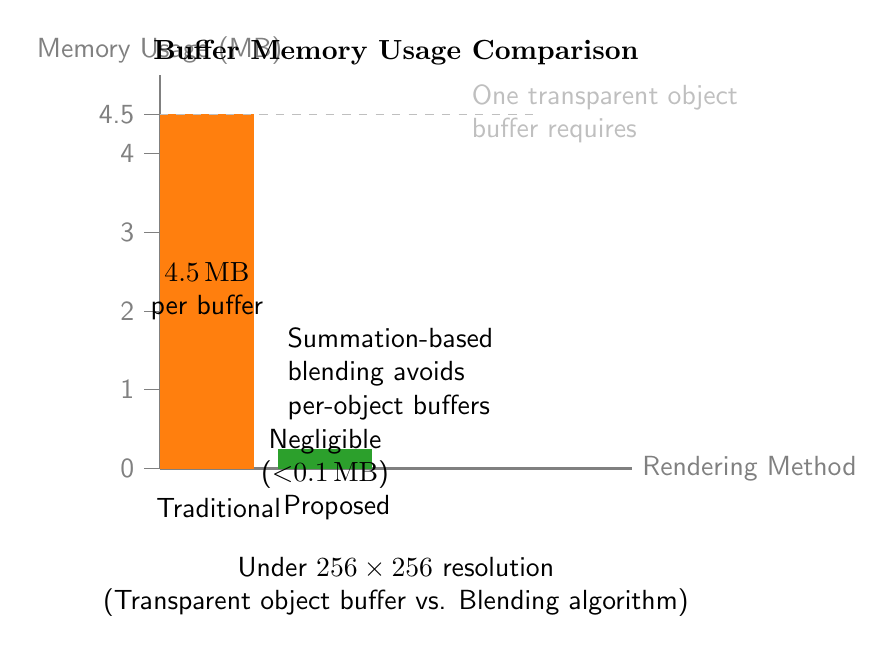
\begin{tikzpicture}[font=\sffamily]
    % Define colors
    \definecolor{buffer}{RGB}{255, 127, 14}  % Orange for traditional buffer
    \definecolor{algorithm}{RGB}{44, 160, 44} % Green for new algorithm
    
    % Chart dimensions
    \def\barwidth{1.2cm}
    \def\barspacing{0.3cm}
    \def\chartheight{5cm}
    \def\chartwidth{6cm}
    
    % Axes
    \draw[thick, gray] (0,0) -- (0,\chartheight) node[above] {Memory Usage (MB)};
    \draw[thick, gray] (0,0) -- (\chartwidth,0) node[right] {Rendering Method};
    
    % X-axis labels
    \node at (\barwidth/2+\barspacing/2, -0.5) {Traditional};
    \node at (3*\barwidth/2+\barspacing/2+\barspacing, -0.5) {Proposed};
    
    % Y-axis ticks
    \foreach \y in {0,1,...,4} {
        \draw[gray] (0,\y) -- (-0.2,\y) node[left] {\y};
    }
    \draw[gray] (0,4.5) -- (-0.2,4.5) node[left] {4.5};
    
    % Memory bars
    \fill[buffer] (0,0) rectangle (\barwidth,4.5) 
        node[midway, black, align=center] {\SI{4.5}{MB}\\per buffer};
    \fill[algorithm] (\barwidth+\barspacing,0) rectangle (2*\barwidth+\barspacing,\chartheight*0.05)
        node[midway, black, align=center] {Negligible\\(\SI{<0.1}{MB})};
    
    % Annotations
    \draw[dashed, gray!50] (0,4.5) -- (0.8*\chartwidth,4.5) 
        node[pos=0.8, anchor=west, align=left] {One transparent object\\buffer requires};
    
    \node[above right, align=left] at (\barwidth+\barspacing, \chartheight*0.1) {
        Summation-based\\blending avoids\\per-object buffers
    };
    
    % Title
    \node[above, font=\bfseries] at (\chartwidth/2, \chartheight) {Buffer Memory Usage Comparison};
    \node[below, align=center] at (\chartwidth/2, -1) {
        Under $256 \times 256$ resolution\\
        (Transparent object buffer vs. Blending algorithm)
    };
\end{tikzpicture}

\end{document}